% floodfusion v1.2 -- preprint.  Build: see paper/README.md (tectonic or latexmk).
% Every number is taken from a committed report under reports/; the source is named in a comment beside it.
% Differences marked "derived" are subtractions of two sourced numbers. Figures: paper/make_figures.py.
\documentclass[10pt,twocolumn,a4paper]{article}

\usepackage[T1]{fontenc}
\usepackage{newtxtext,newtxmath}
\usepackage[a4paper,margin=17mm,top=19mm,bottom=20mm,columnsep=6.5mm]{geometry}
\usepackage{microtype}
\usepackage{booktabs,tabularx,multirow}
\usepackage{graphicx}
\usepackage{xcolor}
\usepackage{amsmath}
\usepackage[font=small,labelfont=bf,skip=4pt]{caption}
\usepackage{subcaption}
\usepackage{tikz}
\usetikzlibrary{arrows.meta,positioning,fit,calc,backgrounds}
\usepackage{enumitem}
\usepackage[numbers,sort&compress]{natbib}
\usepackage{fancyhdr}
\usepackage[colorlinks=true,linkcolor=linkblue,citecolor=linkblue,urlcolor=linkblue]{hyperref}
\usepackage{xurl}

\definecolor{linkblue}{HTML}{1F4E79}
\definecolor{okBlue}{HTML}{0072B2}
\definecolor{okOrange}{HTML}{E69F00}
\definecolor{okPink}{HTML}{CC79A7}
\definecolor{okGreen}{HTML}{009E73}
\definecolor{okVermilion}{HTML}{D55E00}
\definecolor{okYellow}{HTML}{FFD23F}

\newcommand{\tstar}{\ensuremath{\tau^{*}}}
\newcommand{\file}[1]{\nolinkurl{#1}}
\newcommand{\pp}{\,\%}
\setlist{nosep,leftmargin=*}
\setlength{\bibsep}{1pt}
\renewcommand{\bibfont}{\footnotesize}

\pagestyle{fancy}
\fancyhf{}
\fancyhead[L]{\footnotesize T.\ Clerici Jurado --- Labels, thresholds and a blind test}
\fancyhead[R]{\footnotesize Preprint, not peer reviewed}
\fancyfoot[C]{\footnotesize\thepage}
\renewcommand{\headrulewidth}{0.4pt}

\hypersetup{pdftitle={Labels, Thresholds and a Blind Test: Evaluating Sentinel-1 Flood Segmentation Against
  Independent Copernicus EMS Maps}, pdfauthor={Teo Clerici Jurado}}

\begin{document}

\twocolumn[{%
\begin{center}
  {\LARGE\bfseries Labels, Thresholds and a Blind Test:\\[3pt]
   Evaluating Sentinel-1 Flood Segmentation Against\\[3pt] Independent Copernicus EMS Maps\par}
  \vspace{9pt}
  {\large Teo Clerici Jurado\par}
  \vspace{2pt}
  {\small BSc in AI \& Data Science, H-FARM College / University of Chichester\par}
  \vspace{5pt}
  {\small Code and reports: \url{https://github.com/teo-clerk/floodfusion}\par}
  {\small Interactive Arena: \url{https://teo-clerk.github.io/floodfusion/arena.html}\par}
  \vspace{2pt}
  {\footnotesize Preprint, 15 October 2026. Release \texttt{v1.2.0}; blind-test models frozen at tag
   \texttt{v1.2.0-freeze}. Not peer reviewed.\par}
\end{center}
\vspace{2pt}
\begin{center}
\begin{minipage}{0.9\textwidth}
\small
\noindent\textbf{Abstract.}
% src: reports/v11_sen1floods11_table.md (0.608), reports/v12_cems_rebuilt.md (CEMS scores), reports/v12_pool_cv.md,
% reports/v12_cems_seen_tests.md (+0.098, Holm p), reports/v12_power.md (0.061), reports/protocol_v1_2.md.
% derived: 0.080 and 0.023 = row 21 - TerraMind at own and cross-fitted thresholds (unrounded, reports/v12_pool_cv.md).
Flood-segmentation models for Sentinel-1 synthetic aperture radar (SAR) are usually ranked by cross-validation on
benchmark chips whose labels share sensors, dates and definitions with the model inputs. We measure how far such
scores carry to operational reference maps: Copernicus Emergency Management Service (CEMS) rapid-mapping
delineations of 38 flood activations from 2023 to 2026, drawn on non-Sentinel radar satellites, against which every
model is applied, without training on these events, at its own calibrated threshold. A gated cross-attention SAR--optical fusion model that
scores 0.608 IoU in leave-one-event-out cross-validation on Sen1Floods11 scores 0.266 on these maps, below a physics
baseline (0.373); the same architecture trained on Kuro Siwo's flood labels scores 0.407, and its optical input
makes no detectable difference. Our v1.2 model adds a seasonal Sentinel-1 reference (same orbit, one year earlier)
and is developed on a pool of 7,006 chips from 138 floods (Kuro Siwo and GEOID-Flood); it scores 0.417 IoU (AP
0.598).
TerraMind-base adapted to the same labels with LoRA, a siamese pre/post-event input, its DEM modality and an equal
tuning budget scores 0.405 (AP 0.583). The 0.080 IoU lead our model held in grouped cross-validation was mostly
threshold transfer: at thresholds fitted on the other groups it shrinks to 0.023. Copernicus's operational Global
Flood Monitoring (GFM) ensemble scores 0.321 on the 34 activations it covers, where our model scores 0.419 (a gap
of $+0.098$, Holm $p = 0.001$ in an exploratory sign-flip analysis). Because this benchmark had been seen during
development, all of these comparisons are exploratory. The confirmatory test is preregistered: every eligible CEMS
flood activation from EMSR899 on is scored by models frozen at a git tag, and the hashes of the sealed scores are
committed to a hash-chained ledger until 20 activations in 15 clusters are scored, or until the end of 2027. Under
independence assumptions, that detects a mean gap of about 0.06 IoU per activation, and 0.07 per cluster, with 80\pp{}
power. We also report two errata in our earlier results; in a post-hoc re-run, one of them reversed our previous
comparison with TerraMind.

\vspace{4pt}
\noindent\textbf{Keywords:} flood mapping; Sentinel-1; synthetic aperture radar; Copernicus Emergency Management
Service; geospatial foundation models; TerraMind; preregistration; blind test
\end{minipage}
\end{center}
\vspace{10pt}
}]

% =====================================================================================================================
\section{Introduction}

Floods are the hazard whose mapping depends most on radar: the weather that floods a valley is the weather that
clouds it, and the C-band synthetic aperture radar (SAR) on Sentinel-1 sees the ground through cloud, day and night.
Two Copernicus services map floods operationally. Rapid mapping by the Emergency Management Service (CEMS) produces
on-demand delineations for each activation, drawn by analysts on satellite imagery ranging from very-high-resolution
commercial images to Sentinel data~\citep{cems2026rapidmapping}. The Global Flood Monitoring (GFM) product runs an ensemble of three algorithms
on every Sentinel-1 acquisition, worldwide and automatically~\citep{salamon2021gfm,krullikowski2023gfm}.
Deep-learning segmentation models trained on benchmark data sets---Sen1Floods11~\citep{bonafilia2020sen1floods11},
Kuro Siwo~\citep{bountos2024kurosiwo} and, recently, GEOID-Flood~\citep{chiriaco2026geoid}---and geospatial
foundation models such as TerraMind~\citep{jakubik2025terramind} promise to do better.

These promises are mostly measured by cross-validation on benchmark chips. Spatial dependence between training and
test data is known to inflate such estimates~\citep{roberts2017cv,ploton2020spatial,meyer2022maps}, and flood
benchmarks add couplings of their own: Sen1Floods11's labels were drawn mostly on the Sentinel-2 image that a fusion
model also receives, and they mark water on a date rather than flood. Recent comparisons also suggest that the encoder
matters less than its reputation. PANGAEA finds that foundation models do not consistently outperform supervised
baselines~\citep{marsocci2024pangaea}; GEOID-Flood reports a consistent but modest advantage for
them~\citep{chiriaco2026geoid}; and in a global evaluation of fine-tuned TerraMind, a U-Net reached higher recall
than every TerraMind configuration, at slightly lower accuracy and precision~\citep{tulbure2025floodsnet}.

We ask three questions. \textbf{(Q1)} How far do cross-validation scores carry to independent operational maps?
\textbf{(Q2)} Does a task-specific model with radar context beat a fairly adapted foundation model, and the operational
GFM product? \textbf{(Q3)} How can such a claim be tested without the test set shaping the model? We address Q1, and
Q2 descriptively, on a benchmark of 38 CEMS flood activations from 2023--2026, fixed by a preregistered rule before
any model was scored on it. That benchmark was seen during development, so our answers to Q2 there are exploratory.
A preregistered blind test, now running, will answer Q2 confirmatorily; it is also our answer to Q3. Our
contributions are:
\begin{itemize}
  \item A measured gap between cross-validation and independent operational maps. Sen1Floods11-trained optical models
    fall from about 0.6 IoU in leave-one-event-out cross-validation to 0.27--0.30, below a physics baseline. The
    training data, labels included, move scores far more than the architecture or the optical input
    (Section~\ref{sec:gap}).
  \item A seasonal-context model (v1.2) and a fair foundation-model opponent: TerraMind-base with LoRA, a siamese
    pre/post input, its DEM and an equal tuning budget, trained on the same pool of 138 floods. On the CEMS maps the two
    nearly tie (0.417 vs 0.405). An apparent 0.08 IoU advantage in cross-validation was mostly threshold transfer
    (Sections~\ref{sec:cv}--\ref{sec:cems}).
  \item An exploratory comparison with Copernicus GFM on the floods it covers (0.419 vs 0.321). The gap lies more in
    GFM's fixed decision rule, exclusion mask included, than in how its likelihood ranks pixels
    (Section~\ref{sec:gfm}).
  \item A preregistered blind test on CEMS activations that no model had seen, with hash-committed scores and a power
    analysis (Section~\ref{sec:blind}).
  \item Two errata in our own earlier results (Section~\ref{sec:errata}), and an account of the project's provenance
    and of how an AI coding agent was used to build and audit it (Section~\ref{sec:ai}).
\end{itemize}

% =====================================================================================================================
\section{Related work}

\paragraph{SAR flood mapping.} Operational SAR flood mapping thresholds the low backscatter of calm water, compares the
image with a reference acquisition, and masks terrain where flooding is implausible, for instance by the height above
the nearest drainage (HAND)~\citep{nobre2011hand}. GFM combines three such algorithms into an ensemble flood extent
with a per-pixel likelihood~\citep{salamon2021gfm,krullikowski2023gfm}, and ships an exclusion mask where SAR cannot
see flooding: radar shadow, layover, dense vegetation and built-up areas.

\paragraph{Benchmarks.} Sen1Floods11 pairs Sentinel-1 chips with hand-labelled water from 11
events~\citep{bonafilia2020sen1floods11}. Kuro Siwo provides flood polygons drawn on Sentinel-1 for multi-temporal
flood mapping~\citep{bountos2024kurosiwo}. GEOID-Flood, derived from CEMS activations, spans 219 events in 65
countries, with pre- and post-event Sentinel-1, a pre-event Sentinel-2 composite, a DEM and validated labels that
separate permanent water from flood~\citep{chiriaco2026geoid}.

\paragraph{Foundation models.} TerraMind is an any-to-any generative multimodal model pre-trained on nine geospatial
modalities~\citep{jakubik2025terramind}; TerraTorch packages it, with other geospatial foundation models, for
fine-tuning~\citep{gomes2025terratorch}. Low-rank adaptation (LoRA)~\citep{hu2021lora} lets a large encoder adapt on
a small GPU. Where no seasonally matched pre-event image is available, context helps across backbones: on two
held-out US flood events, AlphaEarth embeddings~\citep{brown2025alphaearth} and a DEM each improved single-date SAR
segmentation for four backbones, TerraMind among them~\citep{thasma2026alphaearth}.

\paragraph{Evaluation practice.} We borrow two practices from fields whose evaluation sets are scarce and reused:
spatially grouped validation~\citep{roberts2017cv,meyer2022maps}, and preregistration, in which hypotheses, analyses
and stopping rules are committed before the outcomes that will test them have been observed~\citep{nosek2018prereg}.

% =====================================================================================================================
\section{Data}\label{sec:data}

\subsection{Inputs}
Every input is fetched from Microsoft Planetary Computer~\citep{planetarycomputer2022}, with no account or key. The
inputs are:
\begin{itemize}
  \item Sentinel-1 radiometrically terrain-corrected backscatter $\gamma^0$ (VV, VH) of the post-event pass, and of
    the latest same-orbit pass up to 60 days earlier;
  \item Sentinel-2 L2A bands B3, B8 and B11, with a per-pixel quality from the scene classification;
  \item the Copernicus GLO-30 DEM, from which slope, HAND, the local incidence angle, radar shadow and layover are
    derived;
  \item JRC Global Surface Water~\citep{pekel2016gsw} for permanent water, and ESA WorldCover~\citep{zanaga2022worldcover}
    for analysis.
\end{itemize}
All layers are resampled to one 10\,m UTM grid on the SAR geometry. Training chips are $256\times256$ pixels
(2.56\,km).

\subsection{Training sets}
\textbf{Sen1Floods11} (v1.0, v1.1) supplies hand labels of water. We use them as flood, after removing JRC permanent
water, on 10 of its 11 events; Paraguay's acquisition is missing from the archive. \textbf{Kuro Siwo} (v1.1, v1.2)
supplies flood polygons drawn on radar, for 36 events in 29 groups of events within 100\,km. v1.1 also built
Sen1Floods11-like water labels on the same chips (Section~\ref{sec:gap}). \textbf{GEOID-Flood} (v1.2, revision
\texttt{868407460bf3}) supplies 111 events from before EMSR656 that Kuro Siwo lacks, of which 102 produced chips
(\file{reports/v1_2_deviations.md}). Its class~2 is flood and its class~1 permanent water. A square must have at least
50\pp{} labelled pixels.

The \textbf{v1.2 pool} joins the two flood-label sets. It holds 7,006 chips from 827 stacks of 138 floods, in 81
location groups formed by 100\,km single linkage across both sets. The largest group holds 13.6\pp{} of the windows,
below the 25\pp{} threshold, fixed before any run, for switching to buffered spatial blocks. Cross-validation is
grouped five-fold, and each group is tested once by a model that never saw it.
% src: reports/v12_pool_cv.md header; reports/v1_2_deviations.md (pool probe rows, ingest yields)

\begin{table*}[t]
\centering\small
\caption{Data sets, their roles and their use. ``Seen'' means that the data informed development: only the blind set
can test v1.2's hypotheses.}
\label{tab:data}
\begin{tabularx}{\textwidth}{@{}l l X p{3.9cm} p{3.2cm}@{}}
\toprule
Data set & Role & Labels or content & Size used & Licence \\
\midrule
Sen1Floods11~\citep{bonafilia2020sen1floods11} & training (v1.0, v1.1) & hand-labelled water, drawn mostly on Sentinel-2
  & 10 events & none declared; not redistributed \\
Kuro Siwo~\citep{bountos2024kurosiwo} & training (v1.1, v1.2) & flood polygons drawn on Sentinel-1
  & 36 events, 29 groups & CC BY (data), MIT (code) \\
GEOID-Flood~\citep{chiriaco2026geoid} & training (v1.2) & flood and permanent water, validated
  & 102 events before EMSR656 & CC BY 4.0 \\
v1.2 pool & training, CV & flood minus permanent water & 7,006 chips, 138 floods, 81 groups & --- \\
CEMS 2023--26 & evaluation (seen) & analyst delineations on non-Sentinel imagery
  & 38 activations, 30 clusters, 75 pairs & \copyright{} EU, CEMS terms \\
Copernicus GFM & comparator & ensemble flood extent and likelihood & 34 activations, 26 clusters
  & \copyright{} EU, CEMS terms \\
Blind set (EMSR $\geq$ 899) & confirmatory test & as CEMS & accruing & \copyright{} EU, CEMS terms \\
\bottomrule
\end{tabularx}
\end{table*}

\subsection{The CEMS 2023--26 benchmark}\label{sec:benchmark}
v1.1's preregistered protocol fixed the benchmark before any v1.1 model was trained.
% src: reports/protocol_v1_1.md §2.3; DATA_CARD.md (CEMS benchmark); reports/v1_1_erratum.md (90 pairs, 605 stacks)
A census of codes EMSR656--EMSR898 found 233 public activation records, 86 of them floods. One rule applied to every
delineation product:
\begin{itemize}
  \item all of its source images are non-Sentinel: radar such as COSMO-SkyMed, PAZ, RADARSAT-2, TerraSAR-X or ICEYE,
    or very-high-resolution optical such as Pl\'eiades or WorldView;
  \item its package is published;
  \item a Sentinel-1 acquisition lies within $\pm24$\,h of its latest image and covers at least half of its extent;
  \item a same-orbit pre-event acquisition exists.
\end{itemize}
44 activations with 117 areas of interest (AOIs) qualified. Each activation keeps at most four AOIs, and each AOI at
most 16 tiles, drawn by a seeded generator blind to the flood and to every model. That leaves 90 (product, pass)
pairs on 605 tiles. A pixel is scored if it lies inside the product's observed region, has valid SAR and is outside
permanent water.

The \emph{primary stratum} holds the products drawn on radar satellites: the conservative test for an optical input.
Excluding EMSR664 (Forl\`i, a case study before v1.1) leaves 38 activations, with 75 pairs and 3,395\,km$^2$ (original tiles) of
mapped flood. Of these pairs, 34 were drawn on very-high-resolution images (CEMS class VHR2) and 41 on coarser
images (class HR+). One storm can trigger several activations, so activations within 100\,km and 60 days of each
other (single linkage) form clusters: 30 of them. Every result is reported at both unit definitions.

\subsection{Copernicus GFM as a comparator}\label{sec:gfmdata}
We read GFM from the EODC STAC catalogue, anonymously.
% src: DATA_CARD.md (GFM coverage); reports/v1_2_deviations.md (disclosures, probes); reports/v12_cems_rebuilt.json
For each pair we take the GFM item of the exact post-event Sentinel-1 frame, matched by acquisition start time, and
resample its ensemble flood extent (binary) and ensemble likelihood (0--100) onto the tile grid by nearest neighbour.
GFM is never a model input.
\begin{itemize}
  \item \textbf{Coverage.} 557 of the 605 tiles have a GFM product. Eight pairs have none: six are Sentinel-1C frames
    from before GFM began processing Sentinel-1C in October 2025, and two are Sentinel-1A frames.
  \item \textbf{Versions.} The tiles span GFM v3.1.0 (328), v4.0.0 (24) and v4.1.0 (205).
  \item \textbf{Units.} A unit counts for GFM only where GFM covers at least 95\pp{} of its scored pixels, so that missing
    GFM pixels do not count as misses. 69 of the 75 primary pairs qualify, giving 34 activations in 26 clusters.
\end{itemize}

% =====================================================================================================================
\section{Methods}\label{sec:methods}

\subsection{Models}
The physics baseline uses no learning. Every learned model shares one training recipe and one decision rule
(Section~\ref{sec:training}).

\paragraph{Physics baseline (row 2).} A tile-adaptive backscatter threshold is combined with a change term against the
pre-event pass and with terrain masks (HAND, slope, radar shadow and layover, permanent water). One offset is set on
Sen1Floods11 validation data.

\paragraph{SAR U-Net (row 4).} A U-Net~\citep{ronneberger2015unet} on Sentinel-1 backscatter alone. It reads no
terrain and no optical input.

\paragraph{Gated cross-attention fusion (row 9).} Two encoders (64--512 channels, GroupNorm) read, respectively, the SAR
stack with terrain (slope, $\log(1{+}\mathrm{HAND})$, local incidence) and the optical bands (B3, B8, B11, MNDWI). The
SAR stack has five channels: VV and VH after and before the event, and their VV difference. At 1/8 resolution the
optical features query the SAR features through eight attention heads. A learned per-pixel gate
$g=\sigma\big(\mathrm{MLP}([q;F_o;F_s])\big)\in[0,1]$, a function of the optical quality $q$ and both feature maps,
adds the result to the SAR stream:
\begin{equation}
  F = F_s + g \odot \mathrm{Attn}\big(Q = F_o,\, K = F_s,\, V = F_s\big).
\end{equation}
With the gate closed, the output is exactly that of the network's own SAR-and-terrain path. Missing optical is a
learned embedding, never zeros, and per-sample modality dropout ($p=0.5$) trains the SAR-only path. A U-Net decoder (256 to 32 channels)
produces the flood logits.

\paragraph{v1.2: seasonal context (row 21).} The seasonal reference lets the model ask not only \emph{is this pixel
water?} but \emph{is this water unusual for this place and season?} A sidecar layer holds it: the median, in linear power,
of every same-orbit Sentinel-1 acquisition within $\pm30$ days of the same date one year earlier, taken over at least
three scenes. It contributes three channels, VV and VH of the seasonal reference and VV after the event minus VV
seasonal (in dB), normalised with fixed data-set statistics. They enter the SAR-and-terrain encoder with an
availability channel. Where a stack has no reference, the model substitutes a learned constant per channel, and
context dropout ($p=0.3$) trains that case. The reference exists for 731 of the 827 pool stacks (88\pp{}) and for 595
of the 605 CEMS tiles (98\pp{}).
% src: src/floodfusion/data/seasonal.py, data/sidecars.py, models/segmenter.py (ContextFloodSegmenter);
% reports/v1_2_deviations.md (pool sidecars; known limitations)
The motivation came from v1.1's diagnostics. On Sen1Floods11 the recent pre-event pass, 5--24 days before the image,
was often already flooded. Replacing it with the seasonal reference lifted the physics baseline by $+0.175$ IoU on
Sen1Floods11 and by $+0.087$ on Kuro Siwo. It did not help on CEMS (0.340 vs 0.371, v1.1 tiles), whose recent reference had been
chosen to precede the activation.
% src: README.md (v1.1, "The seasonal reference"); reports/v11_kurosiwo_table.md; reports/cems_benchmark.md (rows 2, 2s)
An AlphaEarth context (rows 20 and 22) was planned and deferred, before any context model was trained: reading the
embeddings from the public mirror took minutes per band and failed under parallel requests.

\paragraph{Fair TerraMind (row 24).} v1.1's TerraMind saw a single date through a frozen encoder. The v1.2 opponent is
TerraMind-1.0-base~\citep{jakubik2025terramind}, used through TerraTorch~\citep{gomes2025terratorch}: the largest
variant in a size rule fixed beforehand for an 8\,GB GPU. TerraMind-large was not tried.
% src: src/floodfusion/models/terramind.py, models/lora.py; reports/v12_tm_probe.json; reports/protocol_v1_2.md
\begin{itemize}
  \item \textbf{Siamese input.} One encoder runs twice with shared weights. The post-event pass reads Sentinel-1 VV
    and VH, Sentinel-2 B3, B8 and B11 where usable (clouded pixels set to the pre-training mean) and the GLO-30 DEM,
    TerraMind's native terrain modality. The pre-event pass reads Sentinel-1 alone.
  \item \textbf{Adaptation.} LoRA~\citep{hu2021lora} of rank 8 ($\alpha=16$) adapts the attention projections. The
    LoRA update starts at zero, so at initialisation the encoder is the pre-trained one.
  \item \textbf{Head.} The tokens of blocks 3, 6, 9 and 12 of both passes are concatenated, reshaped into a pyramid
    and decoded by a U-Net decoder (256 to 32 channels).
  \item \textbf{Shared rules.} Modality dropout is row 9's, and the neck and decoder run once per batch (the erratum~1
    fix, Section~\ref{sec:errata}).
\end{itemize}
Size and adaptation followed a rule logged before any result. Base with LoRA was to be used unless a timing probe
projected more than 3\,h per pooled cross-validation run, with base frozen and then small with LoRA as the
fallbacks. The probe projected 0.40\,h at 2.9\,GB of peak reserved memory, so base with LoRA was used. It trains
20.4\,M parameters, against 18.2\,M for row 9. Figure~\ref{fig:arch} shows both architectures.

\begin{figure*}[t]
\centering
\begin{tikzpicture}[
    font=\scriptsize, >={Stealth[length=4pt,width=3pt]},
    inp/.style={draw=#1, fill=#1!10, rounded corners=2pt, align=left, inner sep=2.5pt, text width=3.75cm,
                minimum height=0.62cm},
    blk/.style={draw=black!65, fill=black!3, rounded corners=2pt, align=center, inner sep=2.5pt},
    lab/.style={font=\footnotesize\bfseries, anchor=west}]
  % ---------------- (a) v1.2 -----------------
  \node[lab] at (-0.1, 0.55) {(a) v1.2: fusion with seasonal context (row 21)};
  \node[inp=okBlue,   anchor=north west] (sar) at (0,0)       {\textbf{Sentinel-1} (5): VV, VH after and before; $\Delta$VV};
  \node[inp=okGreen,  anchor=north west] (ter) at (0,-0.72)   {\textbf{Terrain} (3): slope, $\log(1{+}$HAND$)$, local incidence};
  \node[inp=okPink,   anchor=north west] (ctx) at (0,-1.44)   {\textbf{Seasonal context} (3\,+\,1): VV, VH a year earlier; VV after $-$ seasonal; available?};
  \node[inp=okOrange, anchor=north west] (opt) at (0,-2.6)   {\textbf{Sentinel-2} (4): B3, B8, B11, MNDWI; per-pixel quality};
  \node[blk, text width=2.35cm, minimum height=1.95cm, anchor=north west] (encs) at (4.55,-0.02)
        {SAR + terrain + context encoder\\[1pt] 64--512 ch., GroupNorm};
  \node[blk, text width=2.35cm, minimum height=0.62cm, anchor=north west] (enco) at (4.55,-2.6)
        {optical encoder\\ 64--512 ch.};
  \node[blk, text width=4.3cm, minimum height=3.2cm, anchor=north west] (fuse) at (7.55,-0.02)
        {\textbf{gated cross-attention} at 1/8 resolution\\[3pt]
         $F = F_s + g \odot \mathrm{Attn}(Q{=}F_o, K{=}F_s, V{=}F_s)$\\[3pt]
         $g=\sigma(\mathrm{MLP}([q;F_o;F_s]))$ per pixel;\\ $g=0$: exactly the SAR-and-terrain path;\\
         missing optical: learned embedding;\\ modality dropout 0.5, context dropout 0.3};
  \node[blk, text width=1.85cm, minimum height=3.2cm, anchor=north west] (dec) at (12.35,-0.02)
        {U-Net decoder\\ 256--32 ch.};
  \node[blk, text width=2.45cm, minimum height=3.2cm, anchor=north west, fill=okBlue!8, draw=okBlue] (out) at (14.7,-0.02)
        {calibrated probability\\ (prior correction, temperature or Platt)\\[3pt] flood if $p > \tau^{*} = 0.25$,\\ for $r=3$};
  \foreach \n in {sar,ter,ctx} \draw[->] (\n.east) -- (\n.east -| encs.west);
  \draw[->] (opt.east) -- (enco.west);
  \draw[->] (encs.east) -- node[above, pos=0.42] {$K,V$} (encs.east -| fuse.west);
  \draw[->] (enco.east) -- node[above, pos=0.5] {$Q$} (enco.east -| fuse.west);
  \draw[->] (fuse.east) -- (dec.west);
  \draw[->] (dec.east) -- (out.west);
  % ---------------- (b) TerraMind-fair -----------------
  \begin{scope}[yshift=-4.45cm]
  \node[lab] at (-0.1, 0.55) {(b) Fair TerraMind: TerraMind-1.0-base + LoRA, siamese (row 24)};
  \node[inp=okBlue, anchor=north west, minimum height=1.1cm] (post) at (0,0)
        {\textbf{After the event}: Sentinel-1 VV, VH; Sentinel-2 B3, B8, B11 where usable; GLO-30 DEM};
  \node[inp=okBlue, anchor=north west] (pre) at (0,-1.55) {\textbf{Before the event}: Sentinel-1 VV, VH};
  \node[blk, text width=2.35cm, minimum height=1.1cm, anchor=north west] (tm1) at (4.55,0)
        {TerraMind-base encoder\\ (frozen) + LoRA $r{=}8$};
  \node[blk, text width=2.35cm, minimum height=0.62cm, anchor=north west] (tm2) at (4.55,-1.55)
        {same encoder};
  \draw[<->, dashed, black!55] (tm1.south) -- node[right, align=left] {shared\\ weights} (tm2.north);
  \node[blk, text width=4.3cm, minimum height=2.17cm, anchor=north west] (cat) at (7.55,0)
        {tokens of blocks 3, 6, 9, 12 of both passes\\ concatenated ($2\times$ width)\\[3pt]
         neck: tokens $\rightarrow$ image $\rightarrow$ pyramid\\[3pt] decoder learns the change itself};
  \node[blk, text width=1.85cm, minimum height=2.17cm, anchor=north west] (dec2) at (12.35,0)
        {U-Net decoder\\ 256--32 ch.};
  \node[blk, text width=2.45cm, minimum height=2.17cm, anchor=north west, fill=okBlue!8, draw=okBlue] (out2) at (14.7,0)
        {calibrated probability\\ (same rule)\\[3pt] flood if $p > \tau^{*}$};
  \draw[->] (post.east) -- (tm1.west);
  \draw[->] (pre.east) -- (tm2.west);
  \draw[->] (tm1.east) -- (tm1.east -| cat.west);
  \draw[->] (tm2.east) -- (tm2.east -| cat.west);
  \draw[->] (cat.east) -- (dec2.west);
  \draw[->] (dec2.east) -- (out2.west);
  \end{scope}
\end{tikzpicture}
\caption{The two systems compared in v1.2. Both are trained on the same pool of 138 floods, with the same loss, schedule,
sampler, calibration and threshold rule. (a) Our model reads terrain and a seasonal Sentinel-1 reference beside the
flood image. (b) The fair TerraMind reads its native modalities, including a pre-event image and its DEM. The
comparison is of system against system: what each reads is part of the comparison.}
\label{fig:arch}
\end{figure*}

\subsection{Training, calibration and selection}\label{sec:training}
% src: configs/base.yaml, configs/overlays/kurosiwo.yaml, runs/.../run.json (v1.2 finals); reports/v12_tuning.json;
% reports/v12_selection.json; reports/protocol_v1_2.md Amendment 1; MODEL_CARD.md
\textbf{Recipe.} Every learned model minimises a focal plus Dice loss with AdamW and a warm-up and cosine schedule. It
trains for at most 30 epochs, stopping early (patience 8) on the validation macro IoU, with an effective batch of 16
in bfloat16.

\textbf{Equal tuning budget.} Each family tried the same three learning rates ($3\times10^{-5}$, $10^{-4}$,
$3\times10^{-4}$) on an inner split of fold~0's training groups. Row 9 chose $3\times10^{-4}$, which row 21
inherits without tuning of its own. TerraMind chose $10^{-4}$.

\textbf{Calibration and threshold.} Calibration is fitted on validation data only: an analytic correction of the prior
shift that the sampler introduces, then temperature scaling~\citep{guo2017calibration}, replaced by Platt scaling~\citep{platt1999}
when that lowers the validation log-loss by more than a set margin. A pixel is flooded when its calibrated
probability exceeds $\tau^{*}=1/(1+r)$, with a stated miss-to-false-alarm cost ratio $r=3$, so $\tau^{*}=0.25$.
Because each model's calibration is its own, so is the threshold on its raw score. The pipeline also produces a
conformal recall threshold~\citep{angelopoulos2022crc}, which is not evaluated here.

\textbf{Selection.} The candidates were row 9 and row 21, compared in pooled cross-validation on whole test stacks (the
deployment operator) as macro IoU at $\tau^{*}$ over the 79 groups with flooded pixels; row 21 had to beat row 9 by
more than 0.005. It won, 0.380 to 0.361, better in 49 of the 79 groups. Two inference add-ons had to raise that mean by at least 0.005 and help a majority of
groups:
\begin{itemize}
  \item per-scene self-calibration, a bounded EM prior shift~\citep{saerens2002prior}, changed it by $-0.042$;
  \item a HAND cut at 15\,m changed it by $+0.001$ and helped 30 of the 79 groups.
\end{itemize}
Neither was adopted.

\textbf{Final models.} Each final model trains on four of the five folds (63 groups, 5,605 chips). The fifth fold's
other 17 groups (617 chips) set early stopping, calibration and the deployment prior. Each model has three seeds (42,
43, 44).

\subsection{Metrics and statistics}\label{sec:metrics}
\textbf{IoU per unit.} A unit is an activation or a cluster. Its IoU comes from the confusion counts pooled over its
AOIs, tiles and seeds at each model's own $\tau^{*}$, and the macro average over units is reported. We also report
three companions:
\begin{itemize}
  \item the \emph{oracle} IoU, at each unit's best threshold in hindsight;
  \item the \emph{self-calibrated} IoU, after a per-scene EM prior shift bounded at $|\Delta\mathrm{logit}|\leq2$;
  \item the threshold-free average precision (AP).
\end{itemize}
These three are computed per seed from per-unit histograms of the calibrated probability, then averaged over seeds.
The histograms have 256 bins equally spaced in logit over $[-10, 10]$, so a threshold resolves to 0.078 logit.

\textbf{Tests.} A gap between two models is the mean per-unit difference. We test it with a two-sided sign-flip test, exact
up to 20 units and by Monte Carlo with 200,000 patterns above; every CEMS test here has at least 26 units. $p$-values are Holm-adjusted~\citep{holm1979}
within each unit definition, and a result counts only if it holds at both. Intervals are 95\pp{} bootstrap intervals
over units.

\subsection{Two errata}\label{sec:errata}
% src: reports/v1_1_erratum.md, reports/v1_1_erratum_p4.md, reports/v1_1_erratum2_p4.md, reports/v1_1_erratum2_exposure.md
Both defects came to light during v1.2's planning and data preparation, after v1.1 had been reported. Each is
documented with its evidence, a regression test and a re-measurement.

\textbf{Erratum 1: TerraMind trained without modality dropout.} TerraMind's configuration set modality dropout to
0.5, as for the fusion model, but the training loop applied dropout only to the fusion architectures. TerraMind therefore
trained with $p=0$, so its SAR-only path, which most CEMS pixels need, was barely trained. Its BatchNorm layers also
saw sub-batches of one to three chips. v1.1 had reported fusion beating TerraMind on CEMS (H4) by $+0.031$ per
activation (Holm $p=0.034$) and $+0.039$ per cluster ($p=0.009$). In a post-hoc re-run on the same, already seen
benchmark (unadjusted $p$), TerraMind-small retrained as described rises from 0.226 to 0.299 IoU, and the comparison
reverses: fusion minus TerraMind is $-0.042$ $[-0.065, -0.018]$ per
activation (fusion better on 10 of 38, $p=0.001$) and $-0.043$ per cluster ($p=0.003$). The preregistered verdict
stands as run, and its conclusion is withdrawn.

\textbf{Erratum 2: zero terrain past a DEM tile edge.} GLO-30 tiles declare no nodata value, so where a stack's grid
needed two tiles, the mosaic kept 0\,m beyond the first tile. Slope and HAND read as zero there, and shadow and layover
were not flagged. The defect touched 172 of the 605 CEMS tiles (14.6\pp{} of the benchmark's tile area), 6.4\pp{}
of Kuro Siwo's stack area and 8.6\pp{} of Sen1Floods11's. Rebuilt with the fix, the CEMS tiles move the models that read terrain by
$+0.002$ to $+0.010$ IoU and the others by at most $0.0001$ (Table~\ref{tab:erratum2}). The post-hoc reversal
survives ($-0.033$ per activation, $p=0.005$). Every v1.2 model is trained on rebuilt data and scored on rebuilt tiles.

\begin{table}[t]
\centering\small
\caption{Erratum 2 on the CEMS benchmark: macro IoU at $\tau^{*}$ over 38 activations, on the original and the rebuilt
tiles (\file{reports/v1_1_erratum.md}).}
\label{tab:erratum2}
\setlength{\tabcolsep}{3pt}
\begin{tabular}{@{}l c c c r@{}}
\toprule
Model & Terrain & Original & Rebuilt & Change \\
\midrule
Fusion (Kuro Siwo) & yes & 0.3967 & 0.4070 & $+0.0103$ \\
Fusion (Sen1Floods11) & yes & 0.2575 & 0.2658 & $+0.0083$ \\
Physics baseline & yes & 0.3706 & 0.3725 & $+0.0019$ \\
SAR U-Net (Kuro Siwo) & no & 0.3945 & 0.3946 & $+0.0001$ \\
SAR U-Net (Sen1Floods11) & no & 0.2807 & 0.2808 & $+0.0001$ \\
TerraMind-small, corrected & no & 0.2992 & 0.2992 & $+0.0000$ \\
\bottomrule
\end{tabular}
\end{table}

% =====================================================================================================================
\section{Results}\label{sec:results}

\begin{figure}[t]
\centering
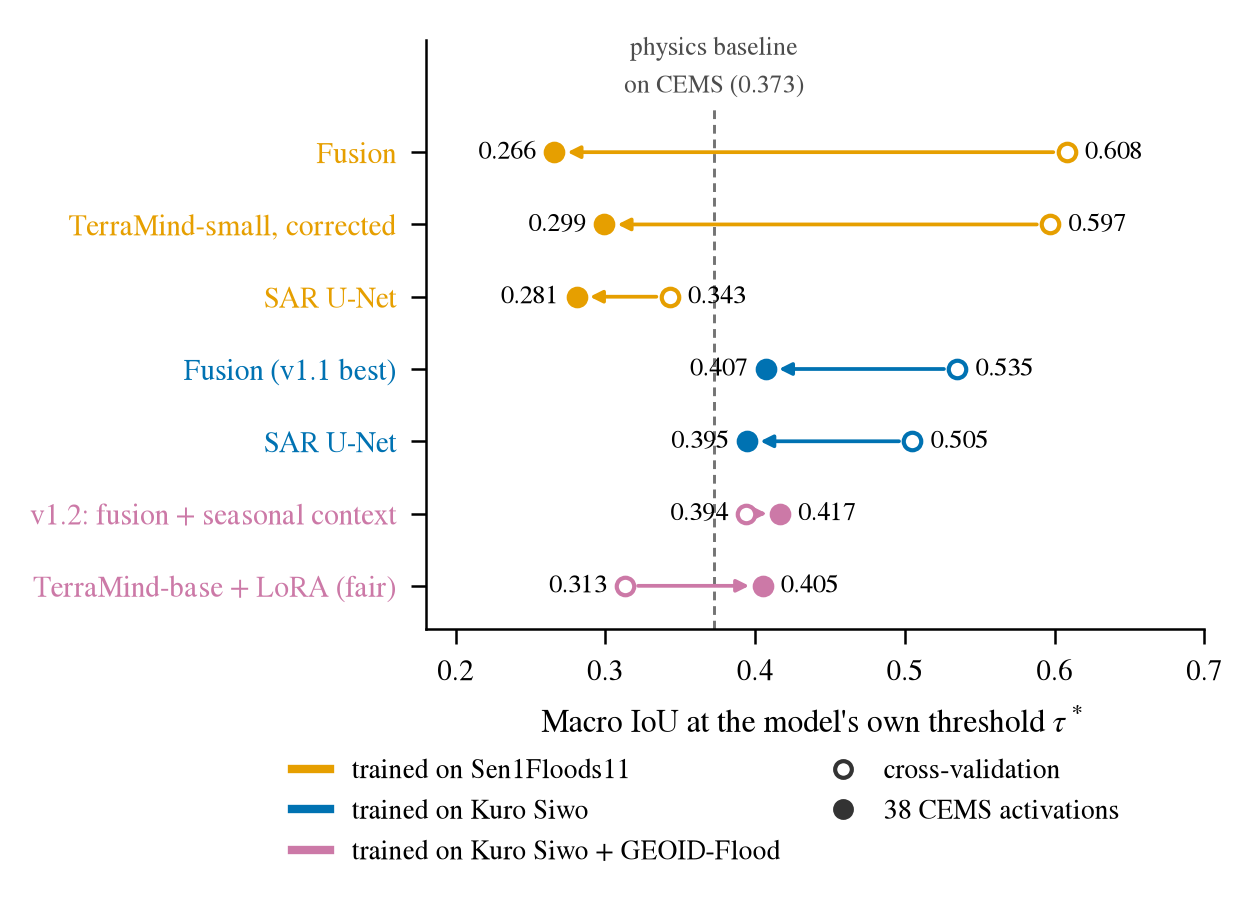
\includegraphics[width=\columnwidth]{figures/cv_vs_cems.png}
\caption{Each model's cross-validation score (open) beside its score on the 38 CEMS activations (filled). The
cross-validation scores are chip-level macro IoU over held-out events or groups: three seeds for Sen1Floods11 and Kuro
Siwo, one for the v1.2 pool. The CEMS scores are per-activation macro IoU, seeds pooled, on the rebuilt tiles. The two
are not the same estimand; the size of the arrows is the point. Sources: \file{reports/v11_sen1floods11_table.md},
\file{v11_kurosiwo_table.md}, \file{v1_1_erratum.md}, \file{v12_pool_cv.md},
\file{v12_cems_rebuilt.json}.}
\label{fig:cvcems}
\end{figure}

\subsection{Cross-validation does not carry to independent maps}\label{sec:gap}
Figure~\ref{fig:cvcems} sets each model's cross-validation score beside its score on the 38 CEMS activations.
\begin{itemize}
  \item \textbf{Sen1Floods11-trained models.} The optical models lose about half of their score or more: fusion falls from
    0.608 in leave-one-event-out cross-validation to 0.266, and the corrected TerraMind-small from 0.597 to 0.299. The
    SAR U-Net falls less (0.343 to 0.281), because its cross-validation score was low to begin with. All three end
    below the physics baseline (0.373).
  \item \textbf{Grouping by event does not prevent this.} On Sen1Floods11, the published within-event split scored the
    fusion model between 0.03 lower and 0.06 higher than leave-one-event-out on the same test chips, depending on the
    seed, and none of these differences was significant after Holm. Both protocols sit far above the CEMS score.
\end{itemize}
% src: reports/v11_sen1floods11_table.md (protocol gap, row 9: -0.027, +0.050, +0.058)

\textbf{The training data matter more.} Trained on Kuro Siwo's flood labels, drawn on radar, the same architectures score
0.395 (SAR U-Net) and 0.407 (fusion) on CEMS. Their cross-validation scores (0.505 and 0.535) overstate them by 0.11
to 0.13 rather than by 0.3.
% derived: 0.505-0.395, 0.535-0.407; 0.608-0.266
v1.1's preregistered test of H1 compares two training recipes on identical Kuro Siwo chips that differ only in the
label definition, which also changes the sampling, the early stopping and the calibration. Flood labels beat water
labels by $+0.059$ IoU per activation (better on 33 of 38, Holm $p<0.001$) and by $+0.062$ per cluster (27 of 30),
on the original tiles. CEMS maps are themselves flood maps, so part of this gain is agreement of definitions.
H1 is the only v1.1 hypothesis that was supported at both unit definitions and still stands. H4 was also supported as
run, but its conclusion is withdrawn (Section~\ref{sec:errata}).
% src: reports/cems_benchmark.md (P3)
With the v1.2 pool, cross-validation no longer overstates the CEMS score: row 21 scores 0.394 in cross-validation and
0.417 on CEMS. The two numbers are different estimands (chips, one seed and 79 groups, against activations, three
seeds and 38 units). We read them as the absence of a large bias, not as an exact match. Part of the agreement may
also be shared conventions: GEOID-Flood's labels, which cover 102 of the pool's 138 floods, are themselves derived
from CEMS delineations~\citep{chiriaco2026geoid}.

\textbf{The optical input adds nothing detectable on independent maps.}
\begin{itemize}
  \item On Sen1Floods11, fusion beat the SAR U-Net by $+0.265$ on all ten events. Its labels were drawn on the
    Sentinel-2 image that the model sees.
  \item On the CEMS activations where optical was usable ($\geq$\,50\pp{} clear; v1.1 tiles), the gain was $+0.038$
    $[-0.024, +0.108]$: not significant over eight activations (Holm $p=0.344$), and no verdict, because seven
    clusters were too few.
  \item Under partial cloud (10--50\pp{} clear, 15 activations, descriptive, v1.1 tiles), the Sen1Floods11-trained fusion model
    scored 0.254 with optical and 0.307 without.
  \item Trained on Kuro Siwo, the fusion model scores 0.397 with optical and 0.398 without (both on the v1.1 tiles).
  \item In the v1.2 pooled cross-validation, row 9 with optical minus row 9 without it at inference is $-0.001$
    $[-0.011, +0.005]$.
\end{itemize}
% src: reports/v11_sen1floods11_table.md (9-4); reports/cems_benchmark.md (P1; Kuro Siwo with/without optical, v1.1 tiles);
% reports/cems_benchmark_strata.md (partial cloud); reports/v12_pool_cv.md (9-11)

\begin{table*}[t]
\centering\small
\caption{Every model on the CEMS 2023--26 benchmark: primary stratum (products drawn on radar), EMSR664 excluded, units
with reference flood, rebuilt tiles. IoU is the macro over units at each model's own $\tau^{*}$, with a 95\pp{}
bootstrap interval over activations. The lower block restricts every model to the units GFM covers on at least
95\pp{} of their scored pixels. GFM's binary product has no $\tau^{*}$; its oracle IoU and AP come from its
likelihood. All of this is exploratory: the benchmark was seen during development
(\file{reports/v12_cems_rebuilt.md}).}
\label{tab:cems}
\setlength{\tabcolsep}{4.2pt}
\begin{tabular}{@{}l l c c c c @{\hspace{14pt}} c c@{}}
\toprule
& & \multicolumn{4}{c}{Per activation} & \multicolumn{2}{c}{Per cluster} \\
\cmidrule(lr){3-6}\cmidrule(l){7-8}
Model & Trained on & IoU at $\tau^{*}$ [95\pp{} CI] & Self-cal. & Oracle & AP & IoU at $\tau^{*}$ & AP \\
\midrule
\multicolumn{8}{@{}l}{\emph{All units: 38 activations, 30 clusters}} \\
v1.2: fusion + seasonal context (row 21) & pool & \textbf{0.417} [0.365, 0.467] & \textbf{0.420} & \textbf{0.468} & \textbf{0.598} & \textbf{0.441} & \textbf{0.628} \\
TerraMind-base + LoRA, fair (row 24) & pool & 0.405 [0.351, 0.455] & 0.362 & 0.446 & 0.583 & 0.429 & 0.612 \\
Fusion, v1.1's best (row 9) & Kuro Siwo & 0.407 [0.355, 0.461] & 0.407 & 0.438 & 0.527 & 0.431 & 0.553 \\
SAR U-Net (row 4) & Kuro Siwo & 0.395 [0.339, 0.448] & 0.393 & 0.429 & 0.525 & 0.414 & 0.547 \\
Physics baseline (row 2) & --- & 0.373 [0.314, 0.430] & --- & --- & --- & 0.405 & --- \\
TerraMind-small, corrected & Sen1Floods11 & 0.299 [0.250, 0.350] & 0.303 & 0.356 & 0.428 & 0.312 & 0.445 \\
SAR U-Net (row 4) & Sen1Floods11 & 0.281 [0.237, 0.322] & 0.248 & 0.314 & 0.317 & 0.298 & 0.328 \\
Fusion (row 9) & Sen1Floods11 & 0.266 [0.219, 0.317] & 0.254 & 0.294 & 0.284 & 0.278 & 0.288 \\
\midrule
\multicolumn{8}{@{}l}{\emph{Units GFM covers: 34 activations, 26 clusters}} \\
v1.2: fusion + seasonal context (row 21) & pool & \textbf{0.419} [0.363, 0.474] & \textbf{0.415} & \textbf{0.467} & \textbf{0.594} & \textbf{0.442} & \textbf{0.623} \\
TerraMind-base + LoRA, fair (row 24) & pool & 0.400 [0.342, 0.457] & 0.359 & 0.441 & 0.573 & 0.425 & 0.602 \\
Fusion, v1.1's best (row 9) & Kuro Siwo & 0.407 [0.346, 0.464] & 0.405 & 0.437 & 0.523 & 0.429 & 0.545 \\
Physics baseline (row 2) & --- & 0.381 [0.315, 0.443] & --- & --- & --- & 0.414 & --- \\
Copernicus GFM (ensemble) & --- & 0.321 [0.253, 0.387] & --- & 0.427 & 0.517 & 0.361 & 0.549 \\
\bottomrule
\end{tabular}
\end{table*}

\subsection{v1.2 against the fair TerraMind in cross-validation}\label{sec:cv}
In pooled cross-validation, row 21 scores 0.394 at its own threshold and the fair TerraMind 0.313, a gap of 0.080
(Table~\ref{tab:cv}).
% src: reports/v12_pool_cv.md (main table; cross-fitted section)
Most of it is threshold transfer. Each fold calibrates its threshold on the next fold's groups. Re-fitting each group's
threshold on all the other groups (cross-fitting, from the stored counts, with no retraining) lifts TerraMind to
0.369 and leaves row 21 at 0.392: a gap of 0.023. At each group's best threshold the gap is 0.024 (0.430 vs 0.406).
Threshold-free, row 21 leads by 0.034 AP (0.651 vs 0.617, fold-level). Row 9, the same model without the seasonal
context, scores 0.383, and 0.382 cross-fitted. The seasonal context's edge over it is single-seed and modest.

\begin{table}[t]
\centering\small
\caption{Pooled grouped five-fold cross-validation, chip level, one seed, 81 groups (79 with a defined IoU). ``Cross-fitted'': each group's
threshold fitted on the other groups' held-out predictions. ``Best'': each group's best threshold in hindsight. AP is
fold-level. The last row is derived from the unrounded values. Source: \file{reports/v12_pool_cv.md}.}
\label{tab:cv}
\setlength{\tabcolsep}{3.6pt}
\begin{tabular}{@{}l c c c c@{}}
\toprule
& \multicolumn{3}{c}{IoU at threshold} & \\
\cmidrule(lr){2-4}
Model & own $\tau^{*}$ & cross-fitted & best & AP \\
\midrule
Row 21 (seasonal context) & 0.394 & 0.392 & 0.430 & 0.651 \\
Row 9 (no context) & 0.383 & 0.382 & 0.425 & 0.632 \\
TerraMind-base + LoRA & 0.313 & 0.369 & 0.406 & 0.617 \\
\midrule
Row 21 $-$ TerraMind & 0.080 & 0.023 & 0.024 & 0.034 \\
\bottomrule
\end{tabular}
\end{table}

\subsection{On 38 CEMS activations: a near tie}\label{sec:cems}
The frozen models were scored once, after the freeze, on the rebuilt tiles (Table~\ref{tab:cems},
Figure~\ref{fig:peract}).
\begin{itemize}
  \item \textbf{Row 21} scores 0.417 IoU at $\tau^{*}$ and 0.598 AP.
  \item \textbf{The fair TerraMind} scores 0.405 and 0.583.
  \item \textbf{v1.1's best model} scores 0.407 and 0.527.
\end{itemize}
Row 21 is better than TerraMind on 24 of the 38 activations ($+0.012$ IoU, $+0.015$ AP), and better than v1.1's best
on 22 of 38 ($+0.010$). With the blind test's own analysis (Table~\ref{tab:seen}), neither gap is significant.
% src: reports/v12_cems_seen_tests.md

\paragraph{Why the cross-validation gap shrank.} Three observations bound the explanation.
\begin{enumerate}[label=(\roman*)]
  \item Threshold transfer accounted for most of the cross-validation gap (Section~\ref{sec:cv}).
  \item On CEMS, TerraMind's threshold transfers well. On the same binned per-seed scores, its IoU at $\tau^{*}$
    (0.407) is 0.039 below its per-activation oracle (0.446), against 0.050 for row 21 (0.418 and 0.468).
  \item The threshold-free gap also shrank, from 0.034 AP in cross-validation to 0.015 on CEMS.
\end{enumerate}
% derived (unrounded, reports/v12_cems_rebuilt.json): oracle - binned tau* = 0.0394 (TerraMind), 0.0497 (row 21);
% AP 0.5981-0.5827 = 0.0154
The cross-validation comparison is single-seed and chip-level, the CEMS comparison three-seed and activation-level,
and 38 activations resolve gaps of this size poorly. We therefore read the result as follows: on these maps, our
task-specific model and the fairly adapted TerraMind-base are not distinguishable at this sample size (Holm $p=0.37$).
Both were trained and scored on data rebuilt with the DEM fix; TerraMind reads DEM gaps inside a window as 0\,m
(Section~\ref{sec:discussion}). The seasonal context's contribution on CEMS is not isolated, because no final model
without it was scored there. Per-scene self-calibration barely helps row 21 (0.418 to 0.420 on the binned scores)
and hurts TerraMind (0.407 to 0.362).

\begin{figure*}[t]
\centering
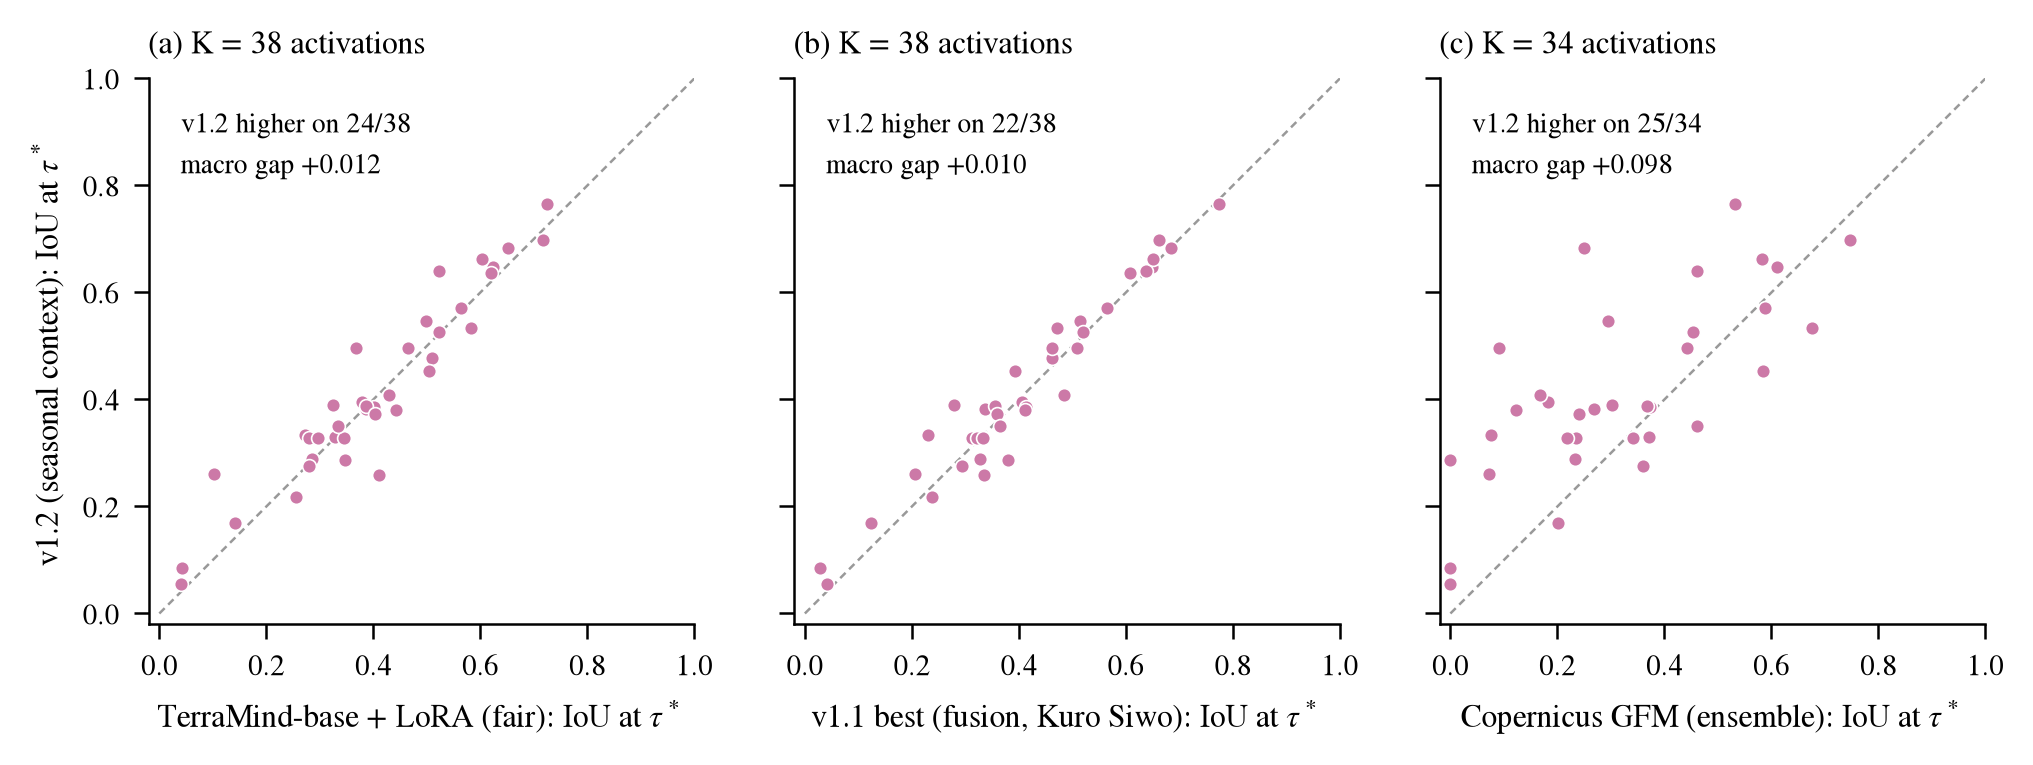
\includegraphics[width=\textwidth]{figures/per_activation.png}
\caption{v1.2's model against (a) the fair TerraMind, (b) v1.1's best and (c) Copernicus GFM: one point per
activation, IoU at each model's own threshold (GFM: its binary ensemble product), seeds pooled. Points above the
diagonal favour v1.2. Panel (c) is restricted to the activations GFM covers. The counts and gaps match
\file{reports/v12_cems_seen_tests.md}. Contains modified Copernicus Emergency Management Service information
(2023--2026).}
\label{fig:peract}
\end{figure*}

\subsection{Copernicus GFM}\label{sec:gfm}
On the 34 activations GFM covers, its ensemble flood extent scores 0.321 IoU, and its likelihood 0.517 AP. Every model
we trained on flood labels scores above it: row 21 0.419, the fair TerraMind 0.400 and v1.1's best 0.407. So does the
physics baseline, at 0.381, which uses no training labels. Only row 21's gap was tested. Row 21 is better on 25 of
the 34 activations, by $+0.098$; per cluster the gap is $+0.081$ (17 of 26). The blind test's analysis code, applied to these seen floods, finds both gaps significant after
Holm ($p=0.0010$ and $p=0.0185$). This is a descriptive result, not a test of H6.
% src: reports/v12_cems_rebuilt.md (GFM block), reports/v12_cems_seen_tests.md (P6)

Much of GFM's deficit lies in its fixed decision rule, exclusion mask included, rather than in how its likelihood
ranks pixels. Thresholded at each activation's best value in hindsight, its likelihood reaches 0.427, 0.106 above its
binary product. This oracle also re-admits pixels inside the exclusion mask, where the likelihood is defined but the
binary product maps no flood. On its binned scores, row 21 gains 0.047 from the same oracle (0.420 to 0.467).
% derived (unrounded, reports/v12_cems_rebuilt.json, GFM-covered units): 0.4270-0.3206; 0.4670-0.4202
Two features of GFM's design also work against it on this reference, and this study does not separate them:
\begin{itemize}
  \item it maps no flood inside its exclusion mask, which includes dense vegetation and built-up areas;
  \item it is produced on a 20\,m grid.
\end{itemize}
A sensitivity analysis restricted to GFM's non-excluded area was planned and has not been run. The pool-trained
models may also benefit from GEOID-Flood's CEMS-derived labels, which share the reference's mapping conventions;
the physics baseline's lead over GFM shows that this does not explain the whole gap. Figure~\ref{fig:quick} shows
one flood as the Arena renders it.

\begin{figure*}[t]
\centering
\begin{subfigure}{0.245\textwidth}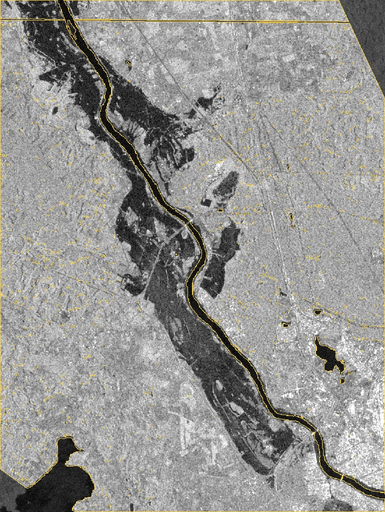
\includegraphics[width=\linewidth]{figures/emsr657_radar.png}\caption{Sentinel-1 VV after the event}\end{subfigure}\hfill
\begin{subfigure}{0.245\textwidth}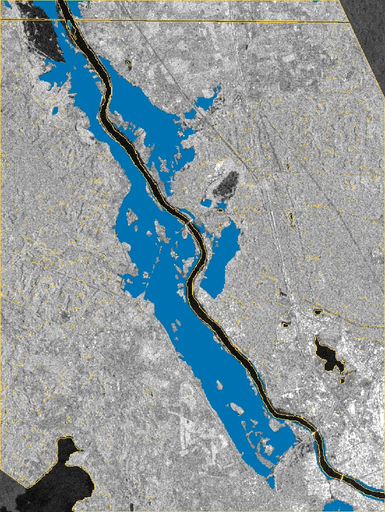
\includegraphics[width=\linewidth]{figures/emsr657_cems.png}\caption{CEMS delineation (reference)}\end{subfigure}\hfill
\begin{subfigure}{0.245\textwidth}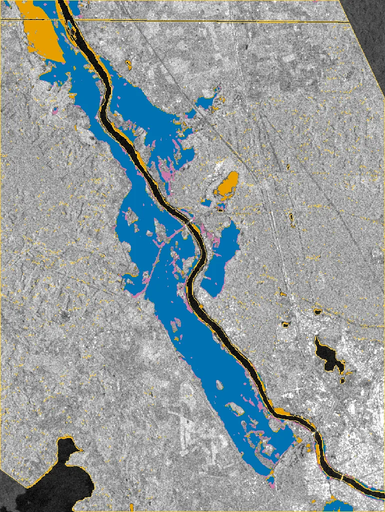
\includegraphics[width=\linewidth]{figures/emsr657_ks_r9_flood.png}\caption{v1.1's best: tile IoU 0.761}\end{subfigure}\hfill
\begin{subfigure}{0.245\textwidth}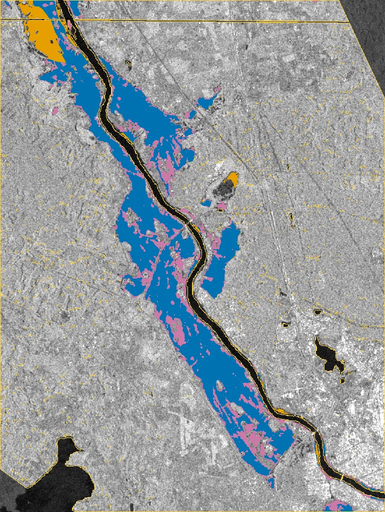
\includegraphics[width=\linewidth]{figures/emsr657_gfm.png}\caption{Copernicus GFM: tile IoU 0.690}\end{subfigure}
\caption{One tile of EMSR657 (AOI~1, tile \file{t02_02}). The CEMS product was drawn on COSMO-SkyMed at 16:22 UTC
on 8 April 2023; the Sentinel-1 pass was at 15:56 UTC; 24.81\,km$^2$ of flood is mapped in the scored region. The
quicklook shows Sentinel-1 VV from $-25$ to 0\,dB. Inside the scored region (yellow outline) the colours are
\textcolor{okBlue}{\textbf{hit}}, \textcolor{okOrange}{\textbf{false alarm}} and \textcolor{okPink}{\textbf{miss}};
outside it the radar is dimmed. The Arena's quicklooks were rendered before the freeze, so they show the v1.1 models
(seed 42) and GFM, not v1.2's model; the tile IoU is not the activation's macro score. Contains modified Copernicus
Sentinel data (2023) and modified Copernicus Emergency Management Service information (2023), \copyright{} European
Union.}
\label{fig:quick}
\end{figure*}

\begin{table}[t]
\centering\small
\caption{The blind test's analysis (\file{floodfusion.blind_analysis}), unchanged, applied to the seen CEMS
floods. ``B $>$ A'': units where v1.2 is better. This is descriptive, not the preregistered test
(\file{reports/v12_cems_seen_tests.md}).}
\label{tab:seen}
\setlength{\tabcolsep}{2.5pt}
\begin{tabular}{@{}l l r r r r r@{}}
\toprule
Test (v1.2 $-$ A) & Unit & K & Gap & B $>$ A & AP gap & Holm $p$ \\
\midrule
\multirow{2}{*}{P5: fair TerraMind} & activ. & 38 & $+0.012$ & 24 & $+0.015$ & 0.3663 \\
                                    & cluster & 30 & $+0.012$ & 19 & $+0.016$ & 0.3293 \\
\multirow{2}{*}{P6: GFM}            & activ. & 34 & $+0.098$ & 25 & --- & 0.0010 \\
                                    & cluster & 26 & $+0.081$ & 17 & --- & 0.0185 \\
\multirow{2}{*}{P7: v1.1's best}    & activ. & 38 & $+0.010$ & 22 & --- & 0.3663 \\
                                    & cluster & 30 & $+0.010$ & 18 & --- & 0.3293 \\
\bottomrule
\end{tabular}
\\[3pt]
\footnotesize Had these been the blind floods, P5 and P7 would read \emph{not supported} and P6 \emph{supported}.
\end{table}

% =====================================================================================================================
\section{The preregistered blind test}\label{sec:blind}
% src: reports/protocol_v1_2.md (sections 1-5, Amendment 1, Corrections); reports/v1_2_deviations.md;
% src/floodfusion/prospective.py; reports/v12_freeze.json; reports/prospective/ledger.jsonl (blind/v1.2); reports/v12_power.md
The CEMS 2023--26 benchmark cannot settle v1.2's questions. It was v1.1's test set, it was seen during v1.2's
development, and public training sets now cover its activations. Because it was seen, the protocol, committed on
13 October 2026 before any v1.2 model was trained, makes only the blind test confirmatory. Before the freeze, a
preview (14 October, after H6 had been registered) scored GFM and the v1.1 models on that benchmark
(\file{reports/v12_cems_preview.md}); v1.2's final models were scored on it only after the freeze.

\subsection{Hypotheses and tests}
Each hypothesis compares B, v1.2's model (row 21), with an opponent A, on the primary stratum, at two unit
definitions:
\begin{itemize}
  \item \textbf{H5 (P5):} B beats the fair TerraMind, both at each model's own threshold and threshold-free.
  \item \textbf{H6 (P6):} B beats Copernicus GFM, on the units GFM covers.
  \item \textbf{H7 (P7):} B beats v1.1's best model.
\end{itemize}
\textbf{Statistic and test.} The statistic is the per-unit gap B $-$ A in macro IoU at $\tau^{*}$, seeds pooled. Each
test is an exact two-sided sign-flip test, Holm-adjusted across P5--P7 within each unit definition. The family always
has three members: a test with fewer than eight units enters it with $p=1$.

\textbf{P5 needs more.} The same must also hold for AP. Its two conditions form one intersection--union test,
$p=\max(p_{\mathrm{IoU}}, p_{\mathrm{AP}})$. This closes a loophole of v1.1, where a win at $\tau^{*}$ reversed at
the oracle threshold. The condition was written on 13 October, before any v1.2 cross-validation run.

\textbf{Verdicts.} A hypothesis is \emph{supported} if its test is significant with a positive gap at both unit
definitions, and \emph{refuted} if it is significant with a negative gap at both. Below eight units at either
definition it has \emph{no verdict}; otherwise it is \emph{not supported}.

\subsection{The blind set}
The blind set is every Copernicus EMS flood activation with code EMSR899 or above, put through v1.1's eligibility rule
unchanged, at most four AOIs per activation. The first activations in that range date from 20 July 2026, and all three
blind flood activations so far (events on 21 August, 25 August and 1 October 2026) predate the freeze of 14 October.
They are blind in a precise sense:
\begin{itemize}
  \item no model was trained or tuned on them;
  \item none was looked at during development;
  \item every one is scored only after the freeze.
\end{itemize}
Only metadata was seen. On 13 October the code, date, category and name of EMSR899--945 were queried to estimate
accrual, and this is disclosed in the protocol. During this paper's fact-check, a reviewing agent also read the cached
activation record of EMSR933: its product list and their statuses, no map, pass or score. This too is logged in the
deviations log. The training activations all precede EMSR656 (2023), and TerraMind's pre-training data date mostly
from 2019--2023. GFM itself is not frozen: the test uses whatever version EODC serves, and records it, and GFM's
ensemble members change in 2027.

\subsection{Freeze, sealing and the ledger}
\begin{figure}[t]
\centering
\begin{tikzpicture}[font=\scriptsize, >={Stealth[length=4pt,width=3pt]},
    stage/.style={draw=black!65, fill=black!3, rounded corners=2pt, align=left, text width=6.9cm, inner sep=3pt},
    key/.style={draw=okBlue, fill=okBlue!8, rounded corners=2pt, align=left, text width=6.9cm, inner sep=3pt},
    node distance=2.4mm]
  \node[key] (f) {\textbf{Freeze} (14 Oct 2026): tag \texttt{v1.2.0-freeze}. 36 files pinned by SHA-256
    (checkpoints, calibrations, $\tau^{*}$), plus the test specification and the census rule.};
  \node[stage, below=of f] (c) {\textbf{Census} of codes $\geq$ EMSR899, in a sweep run by hand (\texttt{make v12-watch}).
    The sweep refuses to run if a pinned checkpoint, a code path or the census rule differs from the freeze.};
  \node[stage, below=of c] (s) {\textbf{Settle}: 30 days after the event, the last fetched copy of the activation
    record is frozen; its SHA-256 enters the ledger.};
  \node[stage, below=of s] (e) {\textbf{Eligibility}: v1.1's rule, unchanged. Then prepare the pair and its DEM,
    seasonal and GFM layers.};
  \node[stage, below=of e] (o) {\textbf{Score} with the frozen models (three seeds each) and GFM.};
  \node[key, below=of o] (l) {\textbf{Seal}: the scores stay outside the repository; their SHA-256 enters the
    committed ledger, where every line carries the SHA-256 of the line before it. A commitment, not a blind.};
  \node[stage, below=of l] (r) {\textbf{Stop} at 20 activations in 15 clusters, or on 31 Dec 2027. \textbf{Reveal}:
    verify every hash and the freeze, then run P5--P7.};
  \foreach \a/\b in {f/c,c/s,s/e,e/o,o/l,l/r} \draw[->] (\a) -- (\b);
\end{tikzpicture}
\caption{The blind test's pipeline (\file{floodfusion.prospective}). The ledger is append-only and hash-chained:
against its committed history, an edited, removed or reordered line is detectable.}
\label{fig:blind}
\end{figure}

The freeze tag pins the models and their calibrations: 36 files are listed by SHA-256 in
\file{reports/v12_freeze.json}. Figure~\ref{fig:blind} shows the pipeline. Before any blind flood was scored, the
whole runner was rehearsed on EMSR664, which lies outside the blind set: one pair, eight tiles, scored by every frozen
model and GFM, sealed and verified against a scratch ledger in 15 minutes.

The seal is a commitment, not a blind. The sealed files are plain JSON on the author's machine, so the seal makes
later changes detectable but does not hide the scores. Sweeps are run by hand, and the runner freezes the last record
it fetched before an activation settles. A sweep should therefore run shortly before each settle time, or products
published late may be missed.

\subsection{Power and stopping}
The stopping rule was raised, before any blind flood was looked at, from 10 activations in 8 clusters to 20 in 15.
Table~\ref{tab:power} gives the reason. Gaps are simulated as i.i.d.\ normal with v1.1's per-activation spread, which
omits clustering. At Holm's smallest level for three tests ($0.05/3$), 20 activations detect a mean gap of 0.061 IoU
at 80\pp{} power, and 10 would detect only 0.096. A verdict needs significance at both unit definitions, and 15
clusters detect 0.072; P5 also needs AP. The end date may come before the counts are reached, with lower power.
The gaps seen on CEMS for P5 and P7 (about 0.01) are far below these.
Unless new floods behave differently, P5 and P7 will most likely end \emph{not supported}. P6's seen gap (0.098) lies
above it.

\begin{table}[t]
\centering\small
\caption{Smallest true mean IoU gap that the blind test detects at 80\pp{} power at Holm's smallest level (0.0167), by
number of activations (\file{reports/v12_power.md}).}
\label{tab:power}
\setlength{\tabcolsep}{4pt}
\begin{tabular}{@{}l c c c c@{}}
\toprule
Per-activation spread (v1.1) & 10 & 15 & 20 & 30 \\
\midrule
SD 0.077 (P4) & 0.096 & 0.072 & 0.061 & 0.048 \\
SD 0.071 (P3) & 0.089 & 0.066 & 0.056 & 0.044 \\
\bottomrule
\end{tabular}
\end{table}

\subsection{Status}
The first sweep ran on 14 October 2026 and took the census to EMSR934. Three blind flood activations had appeared:
\begin{itemize}
  \item EMSR926 (Latvia and Lithuania) and EMSR927 (Nepal) were not eligible under v1.1's rule;
  \item EMSR933 (Crete, event on 1 October) is judged for eligibility when it settles, on 31 October 2026.
\end{itemize}
The Arena shows only counts and statuses until the stopping rule is met.

% =====================================================================================================================
\section{Discussion}\label{sec:discussion}

\paragraph{What moved the scores.}
\begin{itemize}
  \item \textbf{The training data, labels included}: 0.141 IoU on CEMS between the same fusion model trained on
    Sen1Floods11 and on Kuro Siwo;
  \item \textbf{the threshold}: most of a 0.080 gap in cross-validation; on CEMS the two v1.2 models lose 0.039 and
    0.050 IoU against their oracle thresholds;
  \item \textbf{the system}: 0.012 on CEMS between our model and the fair TerraMind, with encoder, inputs and
    context together;
  \item \textbf{the optical input}: about zero.
\end{itemize}
% derived: 0.407-0.266 (rebuilt tiles); oracle - binned tau*: 0.039 (TerraMind), 0.050 (row 21)
As in GEOID-Flood~\citep{chiriaco2026geoid} and PANGAEA~\citep{marsocci2024pangaea}, the choice of encoder moved
scores little; unlike GEOID-Flood, we see no foundation-model advantage. For operational use, labels with flood
semantics and an explicit decision rule mattered more here than the network.

\paragraph{What a fair comparison needs.} A fair comparison needs five things:
\begin{itemize}
  \item the same labels and data;
  \item the same training recipe;
  \item the same tuning budget;
  \item each model's native inputs;
  \item rules fixed before results.
\end{itemize}
It also needs a threshold-free metric beside the thresholded one, because thresholds transfer differently from one
model to another. Our v1.1 comparison failed the recipe condition through a bug (erratum~1). It was caught while
preparing a fair opponent for v1.2.

\paragraph{Reading the GFM comparison.} GFM is built for automated global operation, with conservative exclusions
and one decision rule for every scene. Its likelihood ranks pixels reasonably (AP 0.517). A threshold chosen for
each activation in hindsight would lift it to 0.427, but no such threshold is available in operation. A per-scene
recalibration of our own models did not help in cross-validation either ($-0.042$ for row 21). Adapting a decision
rule to each scene is not free.

\paragraph{Limitations.}
\begin{itemize}
  \item \textbf{Reference maps are products, not ground truth.} CEMS delineations are generalised analyst maps, drawn
    on commercial images (34 of the 75 primary pairs on VHR2-class images, 41 on coarser HR+-class images) taken up
    to 24\,h from the Sentinel-1 pass. Low IoU partly measures the difference between two products.
  \item \textbf{The benchmark is seen and small.} The CEMS 2023--26 benchmark informed development, and 38
    activations resolve gaps of about 0.01 poorly. GEOID-Flood's labels are themselves derived from CEMS
    delineations. The cross-validation is single-seed.
  \item \textbf{The opponent's configuration.} The size rule, fixed for the 8\,GB GPU, stopped at TerraMind-base;
    TerraMind-large was not tried. LoRA adapts only the attention projections. TerraMind's SAR input is our z-scored
    backscatter, adapted by four affine parameters rather than its pre-training normalisation. The band subset and
    necks follow IBM's Sen1Floods11 recipe, and the schedule is row 9's. The equal tuning budget covers only the
    learning rate, whereas row 9's design went through two earlier releases. Missing DEM pixels inside an available
    window read as 0\,m (disclosed before the freeze).
  \item \textbf{Pre-training exposure.} TerraMind's pre-training data date mostly from 2019--2023, so its encoder may
    have seen unlabelled imagery of the benchmark's 2023 events; ``never saw the event'' holds for its decoder.
  \item \textbf{The selection.} The inner validation groups used for tuning serve as test groups in other folds. This
    applies to both families equally, by design.
  \item \textbf{GFM.} The effects of GFM's exclusion mask and its 20\,m grid are not separated. GFM versions are mixed
    on the benchmark, and GFM is not frozen for the blind test.
  \item \textbf{Overlap.} Place overlap between the v1.2 pool and the benchmark was not re-measured. v1.1 found five
    pairs overlapping Kuro Siwo training areas, and dropping them left H1's verdict unchanged.
  \item \textbf{Training data defects.} The v1.1 models were trained on data that carried erratum~2 and were not
    retrained.
  \item \textbf{Timestamps.} Commit dates are set by the author's machine. GitHub first received the protocol and the
    freeze tag on 15 October 2026, before any blind flood was scored; no independent archive holds them yet.
\end{itemize}

% =====================================================================================================================
\section{AI-assisted engineering and reproducibility}\label{sec:ai}

\paragraph{Provenance and the author's role.} The author, Teo Clerici Jurado, wrote the original v1.0 project
specification and defined the project's core research objectives: to test findings made on Sen1Floods11 against real
Copernicus EMS activations, to audit whether the comparison with a foundation model, TerraMind, is fair, and to decide
the main comparison by a preregistered blind test. The specification fixed v1.0's architecture, its ablation grid,
the training recipe and the decision rule. The repository's first commit (\texttt{212e0e6}, 9 October 2026) imported
it unchanged (``as received'' in its message) with a skeleton package, the ablation configurations and a test
specification of 281 test functions. The specification documents were removed from the history before publication
and are not public; the commit holds the package, the configurations and the tests. The author directed the agent
workflow described below: they set each release's goals, reviewed and approved each release's plan, and made the
decisions on data licensing, compute scheduling and publication. The v1.2 protocol, preregistration design included,
was drafted with Claude Code and reviewed and approved by the author; the audits were run by AI subagents. The author
takes full scientific responsibility for the work, its errata and corrections, and this paper.
% src: git show --stat 212e0e6 (root commit; message "import Project 01 curriculum skeleton as received", body
% "exactly as delivered"); git ls-tree 212e0e6: configs/ 15 files, src/ 21, tests/ 16 with 281 test functions

\paragraph{Use of an AI coding agent.} The project was built with Claude Code (Anthropic), an AI coding agent that the
author operated throughout. In line with the generative-AI policies of publishers such as IEEE, NeurIPS and AGU, the
agent is not an author, its use is described here, and the human author is accountable for the results. Under the
author's direction, the agent:
\begin{enumerate}[label=(\roman*)]
  \item searched and summarised the literature, and drafted the v1.2 study design, the protocol text and the analysis
    rules, which the author approved;
  \item implemented the specification and the later releases: the data pipeline, the models, the scorers, the
    blind-test runner and the Arena page;
  \item extended the test suite from the 281 specified test functions to 867;
  \item ran structured review passes with separate agent instances: code, Python, machine-learning engineering and
    security. Their findings were fixed or, where a fix would have changed models already cross-validated,
    disclosed; findings that touched a rule were logged before the result they could affect. The review of the
    blind-test design checked for train--test leakage and found none. These reviewers are instances of the same AI
    system that wrote the code, so they are not independent of it;
  \item traced and measured both errata;
  \item fact-checked the documentation, and this manuscript, against the generated reports;
  \item drafted this manuscript.
\end{enumerate}
The deviations logs record each rule before the result it could affect, and disclose the exceptions: for example,
v1.1's first amendment was written after the Stage A diagnostics of the v1.0 models.

\paragraph{Reproducibility.}
\begin{itemize}
  \item \textbf{Runs and reports.} Every training run records its code commit, whether the tree was clean, and hashes
    of its configuration, manifest and splits. The table builders refuse runs made from different code, mixed data
    sets or mixed test sets.
  \item \textbf{Environment and tests.} The environment is locked with uv. Continuous integration runs the linter and
    the offline test suite on Python 3.11 and 3.12. At this release, 1,091 offline tests pass and 2 are skipped, with
    81.9\pp{} combined statement and branch coverage of the package; tests that need live services are excluded by
    default.
  \item \textbf{The blind test.} Its models, calibrations, thresholds and specification are pinned by SHA-256 at the
    freeze tag.
  \item \textbf{Compute.} Every experiment ran on one laptop GPU (NVIDIA RTX 4060 Laptop, 8\,GB), one job at a time.
\end{itemize}
% src: README.md (Reproduce; table builders); test run at commit ad97913: 1091 passed, 2 skipped, 6 deselected,
% coverage 81.92 %

% =====================================================================================================================
\section{Conclusion}
On the seen CEMS benchmark (exploratory), the training data and the decision rule mattered more than the network:
\begin{itemize}
  \item a task-specific seasonal-context model and a fairly adapted TerraMind-base are not distinguishable over 38
    activations;
  \item both score above GFM's binary product on the floods it covers (0.419 and 0.400 against 0.321; only the first
    gap was tested);
  \item cross-validation on a benchmark whose labels share the model's inputs overstated a model's score by up to
    0.34 IoU.
\end{itemize}
% derived: 0.608-0.266
The decisive comparison is the blind test. Frozen models, hash-committed scores and a fixed stopping rule will decide
H5--H7 on floods that none of the models had seen.

% =====================================================================================================================
\section*{Data and code availability}
The code (MIT licence), the protocols, the deviations logs and every report are at
\url{https://github.com/teo-clerk/floodfusion}. The release is tag \texttt{v1.2.0}, and the blind test's models are
frozen at tag \texttt{v1.2.0-freeze}. The interactive Arena (\url{https://teo-clerk.github.io/floodfusion/arena.html})
shows every model on the same floods. Every input comes from public sources and needs no credentials: Microsoft
Planetary Computer, the CEMS rapid-mapping API, EODC's GFM catalogue, the Kuro Siwo annotations and GEOID-Flood.
Sen1Floods11 declares no licence, so its data, chips and the weights trained on it are not redistributed. Kuro Siwo
(CC BY) and GEOID-Flood (CC BY 4.0) are re-downloaded by the user rather than redistributed, and model weights are
not distributed.

\section*{Acknowledgements}
Contains modified Copernicus Sentinel data (2015--2026), accessed through Microsoft Planetary Computer; Sentinel-1 RTC
processed by Catalyst (CC BY 4.0). Contains modified Copernicus Emergency Management Service information (2023--2026): rapid-mapping delineations and Global Flood Monitoring (GFM)
flood maps, \copyright{} European Union. Copernicus DEM \copyright{} DLR e.V.\ 2010--2014 and \copyright{} Airbus
Defence and Space GmbH 2014--2018, provided under COPERNICUS by the European Union and ESA. JRC Global Surface Water:
EC JRC/Google. ESA WorldCover 2021. TerraMind: IBM and ESA. Kuro Siwo: Orion AI Lab, data CC BY, annotation code
MIT. GEOID-Flood: Chiriaco et al., CC BY 4.0. Claude Code (Anthropic) was used to implement the software and to draft
this manuscript; Section~\ref{sec:ai} describes its use.

{\small
\bibliographystyle{unsrtnat}
\bibliography{references}
}

\end{document}
